\chapter{Tecnologia Wi-Fi direct}
La tecnologia Wi-Fi Direct viene sviluppata dalla Wi-Fi Alliance, e permette di stabilire una comunicazione senza fili tra due dispositivi ( anche di differente natura: Tablet, Pc, TV, ecc… ), senza appoggiarsi ad un Router Wireless, il requisito fondamentale è che almeno uno dei due dispositivo disponga di tale tecnologia.
Wi-Fi Direct si comporta un po´ come la modalità “ad-hoc” nel caso del Wi-Fi semplice ( assegnazione statica dei ruoli di Client e Server) con la differenza che decide dinamicamente quale dispositivo debba fungere da Server e quale da Client., potendo inoltre utilizzare simultaneamente uno smartphone come server e come client.
Oltre che dalla semplicità d'uso, è contraddistinto anche da una contenuta richiesta in termini di risorse energetiche permettendo così una maggior durata della batteria rispetto, ad esempio, all'utilizzo del Bluetooth.


\section{Funzionamento protocollo}
I dispositivi vengono definiti P2P Devices, e possono comunicare tra loro grazie ai P2P Groups.
All’interno di questi gruppi, il dispositivo che funziona come un Access Point ( AP ), cioè il nostro “router” viene definito come P2P Group Owner ( P2P GO ), tutti gli altri dispositivi saranno chiamati P2P Client, e potranno interagire con il P2P GO.
Come detto in precedenza, la decisione di quale dispositivo sarà il GO e quale il Client non è “Statica”, ma al momento della fase di Discover ( fase in cui i dispositivi si cercano ), quando i dispositivi si troveranno e avverrà l’associazione, partirà una sorta di negoziazione in cui si deciderà chi sarà il GO, e solo una volta che sarà stabilito i dispositivi Client potranno unirsi ad esso.

\begin{center}
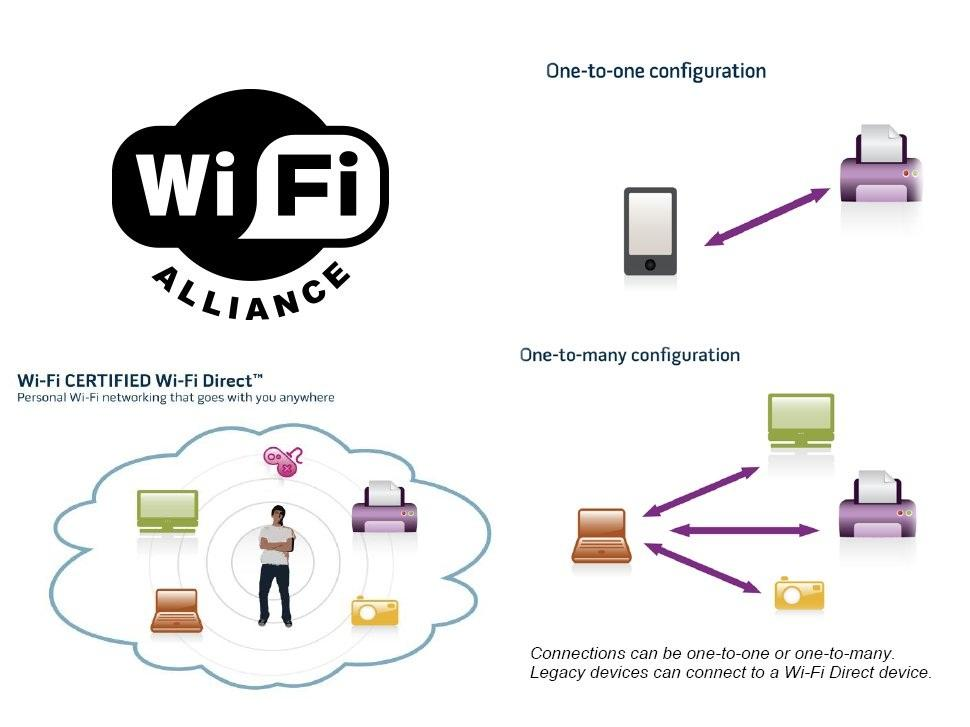
\includegraphics[width=1\textwidth]{imgs/wifi_alliance.jpg}
\captionof{figure}{Possibili utilizzi della tecnologia}\label{wifi_alliance_img}%
\end{center}

Nella figura  \ref{wifi_alliance_img} vengono mostrati i possibili utilizzi di questa tecnologia.
Nella One-to-one configuration notiamo che la connessione avviene tra uno smartphone e una stampante, in questo modo possiamo avere accesso alla stampante per stampare i file di relativo interesse.
Nella One-to-many configuration invece notiamo come la connessione avvenga tra più dispositivi ( in questa configurazione il Laptop sarà Il P2P GO e tutti gli altri i Client ), in questo modo si può interagire col P2P GO per avere accesso agli altri dispositivi, per esempio, dalla fotocamera inviare un file al PC oppure stampare direttamente una foto.
Oppure tramite lo stesso P2P GO si può avere accesso ai file degli altri dispositivi e stamparli inviandoli alla stampante.

\subsection{Formazione del P2P Group Owner}

Come detto in precedenza, perché la comunicazione tra due dispositivi avvenga c’è bisogno che venga instaurato un Group Owner ( GO ).
Wi-Fi Direct permette di creare tre gruppi differenti:

\subsubsection{Gruppo Standard}

In tale caso è necessario che i due dispositivi si trovino tramite la fase di Discover, e successivamente partirà la fase di negoziazione del GO.

\begin{center}
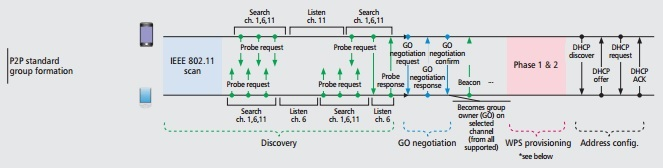
\includegraphics[width=1\textwidth]{imgs/Standard_Group.jpg}
\captionof{figure}{Illustrazione della formazione di un gruppo standard}\label{standard_group_img}%
\end{center}

Come si nota nella Figura \ref{standard_group_img} per prima cosa i P2P Devices selezionano uno dei tre canali ( 1, 6, 11 ) chiamati canali di ascolto.
Successivamente si alterneranno tra due stati: search e listen.
Nello stato di search i P2P Devices inviano un segnale ( di indagine ) chiamato Probe Request nei 3 canali.
Nello stato di listen invece, i P2P Devices saranno in ascolto sul proprio canale, in attesa di questo segnale ( Probe Request ) e saranno pronti a rispondere con il Probe Response.
Una volta che poi i due P2P Devices si sono trovati, inizierà la fase di negoziazione ( GO Negotiation ).
Per stabilire quindi chi sarà il GO e chi il Client, i due P2P Devices si invieranno un valore numerico ( GO Intent value ) tramite il meccanismo three-way handshake (  GO Negotiation Request/Response/Confirm ), e chi dichiarerà il valore più alto diventerà il P2P GO.
Per evitare qualsiasi tipo di conflitto in caso i due P2P Devices dichiarino lo stesso valore, è stato implementato un bit aggiuntivo ( tie-breaker).
Una volta che sono stati stabiliti i ruoli per i due P2P Devices, si passa all’ultima fase, che consiste nello stabilire una connessione sicura usando il Wi-Fi Protected Setup ( WPS Provisioning phase Figura 1.3 ) ed infine il settaggio di un indirizzo IP tramite lo scambio di DHCP.

\subsubsection{Gruppo Autonomous}

\begin{center}
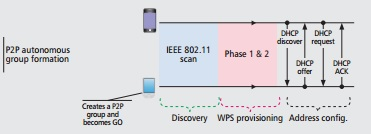
\includegraphics[width=1\textwidth]{imgs/Autonomous_Group.jpg}
\captionof{figure}{Illustrazione della formazione di un gruppo autonomo}\label{autonomous_group_img}%
\end{center}

Come si può notare dalla figura \ref{autonomous_group_img}, un P2P Device può creare autonomamente un P2P Group che diventa immediatamente il P2P GO, istanziandosi su un canale e cominciando a inviare segnali ( beacon ).
Gli altri dispositivi possono trovare tale gruppo con metodi tradizionali di scansione e procedere direttamente alla creazione della WPS Provisioning e all’Address Configuration.

\subsubsection{Gruppo Persistent}

\begin{center}
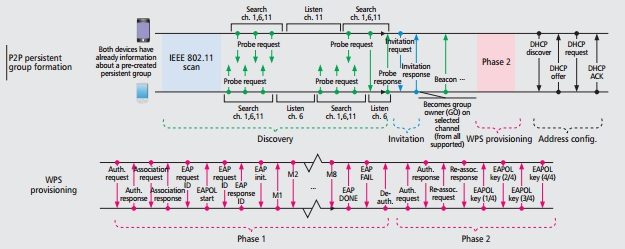
\includegraphics[width=1\textwidth]{imgs/Persistent_Group.jpg}
\captionof{figure}{Illustrazione della formazione di un gruppo persistente}\label{persistent_group_img}%
\end{center}

Come si può notare in figura \ref{persistent_group_img}, un P2P Device può essere in grado di riconoscere un gruppo già formato in precedenza usando i flag del P2P Capabilities presente nel Beacon frame, del Probe Response e del GO Negotiation.
In questo modo, se dopo la fase di Discovery un P2P Device riconosce che tale gruppo era già stato formato in precedenza con lo stesso peer.
Uno dei due P2P Device è in grado di ricreare quel gruppo tramite un processo di invito ( Invitation Procedure ) in modo molto veloce.

\subsection{Sicurezza ( WPS Provisioning )}

Come detto in precedenza, dopo che la fase di Discover è terminata e dopo che la negoziazione è finita, decidendo quindi chi ha il ruolo di P2P Group Owner e chi di Client, parte un ultima ma non meno importante fase, quella del WPS Provisioning.
I dispositivi che implementano Wi-Fi Direct devono implementare anche questo protocollo di sicurezza, in quanto si occupa di creare una connessione sicura tra i due, richiedendo il minimo sforzo all’utente.
Nello specifico, questo protocollo permette di creare una connessione sicura, richiedendo di immettere un determinato codice PIN dalla parte Client, oppure di premere un pulsante in tutti e due i dispositivi.
Per seguire le direttive del WPS, il P2P GO deve implementare il Registrar e il Client l’Enrollee.

\begin{center}
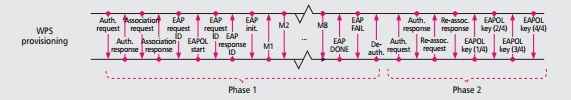
\includegraphics[width=1\textwidth]{imgs/WPS.jpg}
\captionof{figure}{Illustrazione del funzionamento del sistema di sicurezza WPS}\label{wps_img}%
\end{center}

Come possiamo vedere dalla Figura \ref{wps_img}, il WPS è composto da 2 fasi.
Nella prima fase il Registrar è incaricato di generare le credenziali per la connessione (  per esempio: chiave di sicurezza ) e di mandarle all’Enrollee.
Tali chiavi vengono generate col protocollo di sicurezza WPA-2, successivamente criptate tramite un protocollo chiamato AES-CCMP.
Nella seconda fase l’Enrollee ( Client ), si disconnette e si riconnette con le nuove credenziali inviategli dal Register.
Nel caso in cui alla riconnessione tutti e due i dispositivi abbiamo già le credenziali richieste si può procedere all’autenticazione, altrimenti si ripartirebbe dalla fase 1.



\section{Confronto con altre tecnologie}

Fino ad ora abbiamo spiegato nel dettaglio come funziona l’architettura WiFi Direct e abbiamo detto che si occupa di far comunicare due dispositivi senza bisogno di un hotspot, potremo dire quindi che è identico alla tecnologia Bluetooth, invece no, perché ha una grande differenza rispetto a quest’ultima, e cioè una migliore velocità nel trasferire le cose, tutto questo perché Wi-Fi Direct implementa per il trasferimento lo stesso protocollo di Wi-Fi.
Qui di seguito viene riportata una tabella che confronta tale tecnologia con Bluetooth:

\begin{center}
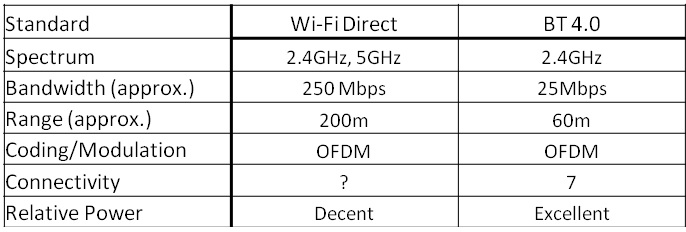
\includegraphics[width=1\textwidth]{imgs/WvsB.jpg}
\captionof{figure}{Wi-Fi Direct e Bluetooth messi a confronto}\label{WvsB_img}%
\end{center}

Per questo le varie applicazioni di questa tecnologia vanno pian piano ad espandersi, fino ad ora lo troviamo impiegato in: 
condivisione di file, sincronizzazione, stampa, video games e tutto ciò senza la necessità di trovare una connessione a internet per comunicare con i device.
Per la parte di applicazione lato condivisione di file lo troviamo nell’applicazione “Wi-Fi Shoot” che è un applicazione molto semplice, che permette una volta che i dispositivi si sono associati di scambiarsi file.
O ancora nell’applicazione “S-Beam” che permette sempre lo scambio di file effettuando un movimento ondulatorio verso l’altro dispositivo.
In ambito videogames invece, viene impiegato dal gioco “Spaceteam” un gioco di squadra in cui bisogna comunicare e dare direttive all’altra persona su cosa deve fare, in questo modo favorisce anche la socializzazione e la sincronizzazione, sia tra persone che tra dispositivi.


\clearpage{\pagestyle{empty}\cleardoublepage}